\chapter{The LHC and the CMS Detector} \label{chap-detector}

\section{The Large Hadron Collider} \label{sec-TheLargeHadronCollider}

\begin{figure}\label{fig-CERNAcceleratorComplex}
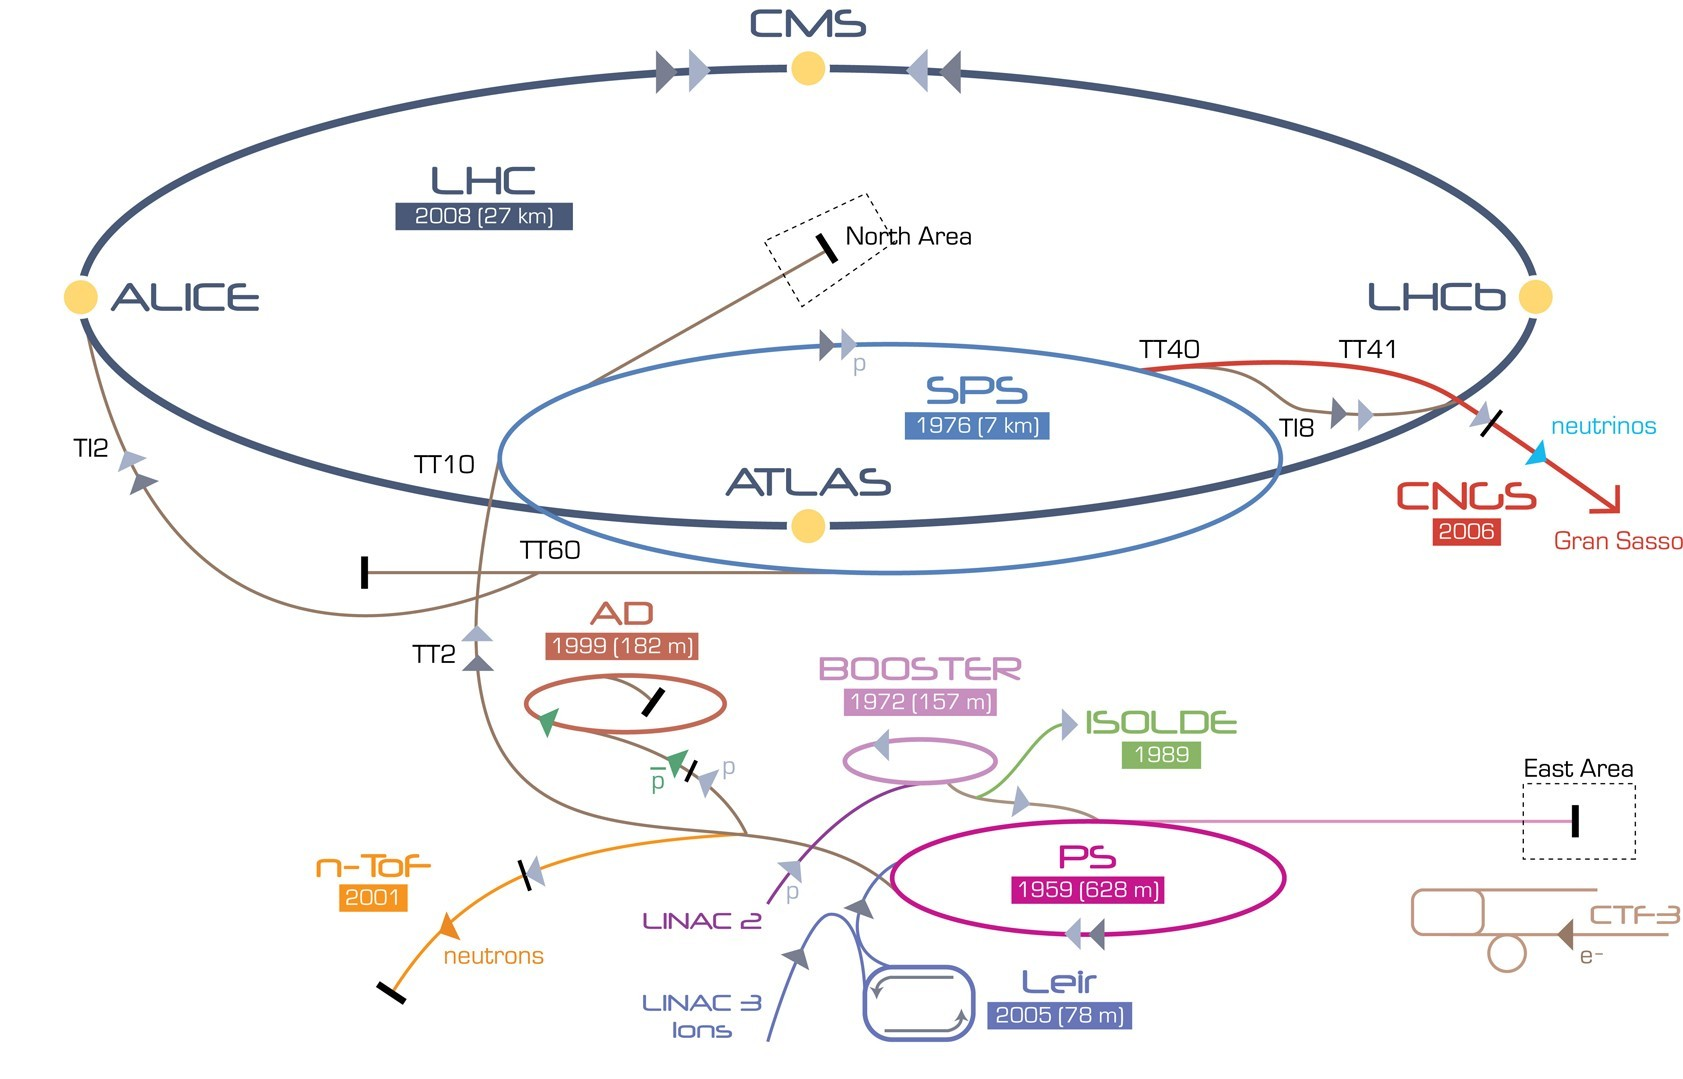
\includegraphics[width=\textwidth]{Figures/CERNAcceleratorComplex.jpg}
\caption{A full schematic of the full CERN accelerator complex \cite{ref-}.}
\end{figure}

\section{The CMS detector} \label{sec-TheCMSDetector}

\begin{figure}\label{fig-CMSDetector}
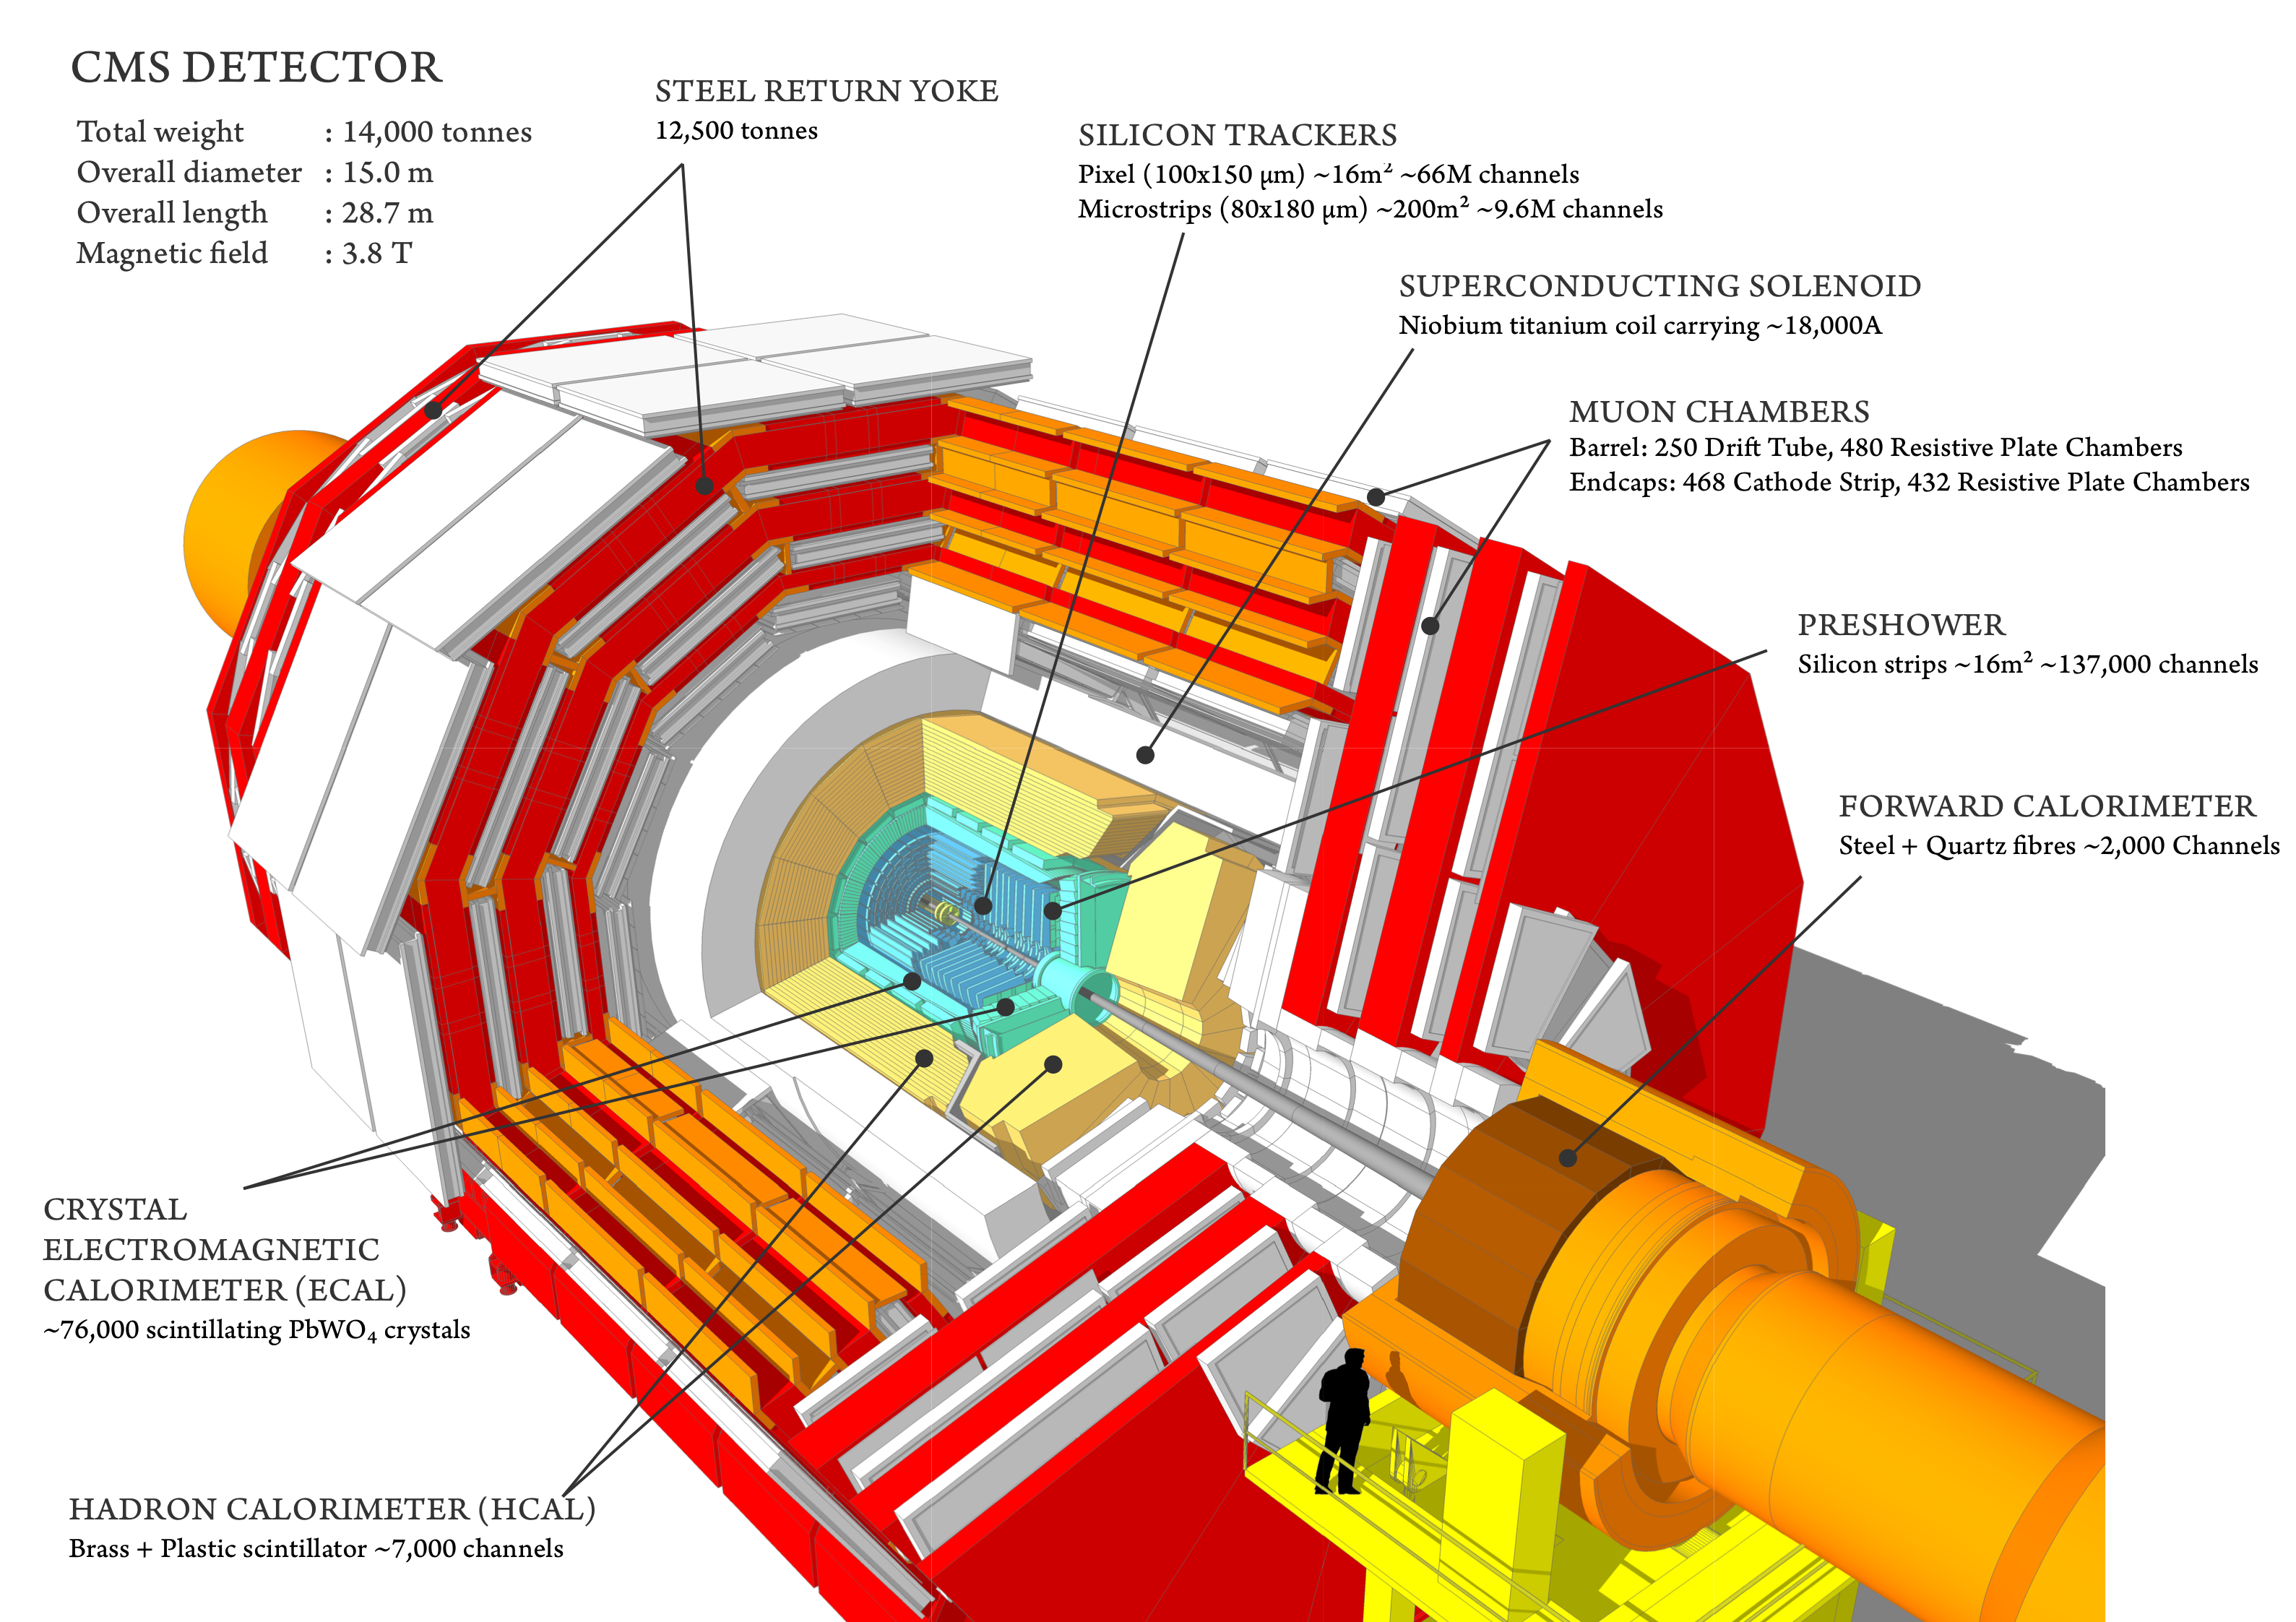
\includegraphics[width=\textwidth]{Figures/CMSDetector.png}
\caption{A cross-sectional view of the CMS detector \cite{ref-}.}
\end{figure}

\subsection{Tracking system} \label{subsec-TrackingSystem}

Figure \ref{fig-Tracker} schematic cross section through the CMS tracker. Each line represents a detector module. Double lines indicate back-to-back modules which deliver stereo hits \cite{CMSexperiment}.

\begin{figure}\label{fig-Tracker}
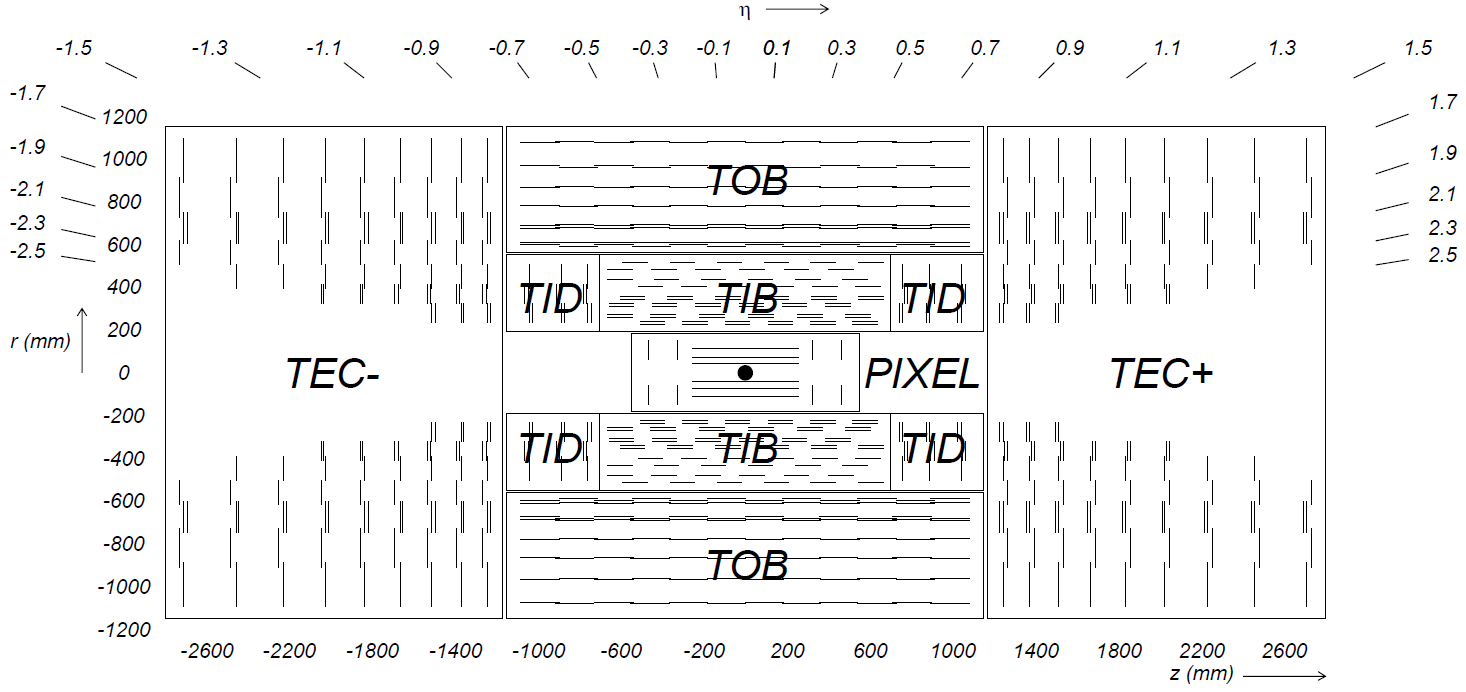
\includegraphics[width=\textwidth]{Figures/Tracker.png}
\caption{The subdetectors of the CMS silicon tracker system: TOB=outer barrel, TIB=inner barrel, TID=inner disc, TEC=endcaps, PIXEL=pixeldetector \cite{ref-}.}
\end{figure}

\subsection{Electromagnetic calorimeter} \label{subsec-ElectromagneticCalorimeter}

\begin{figure}\label{fig-ECAL}
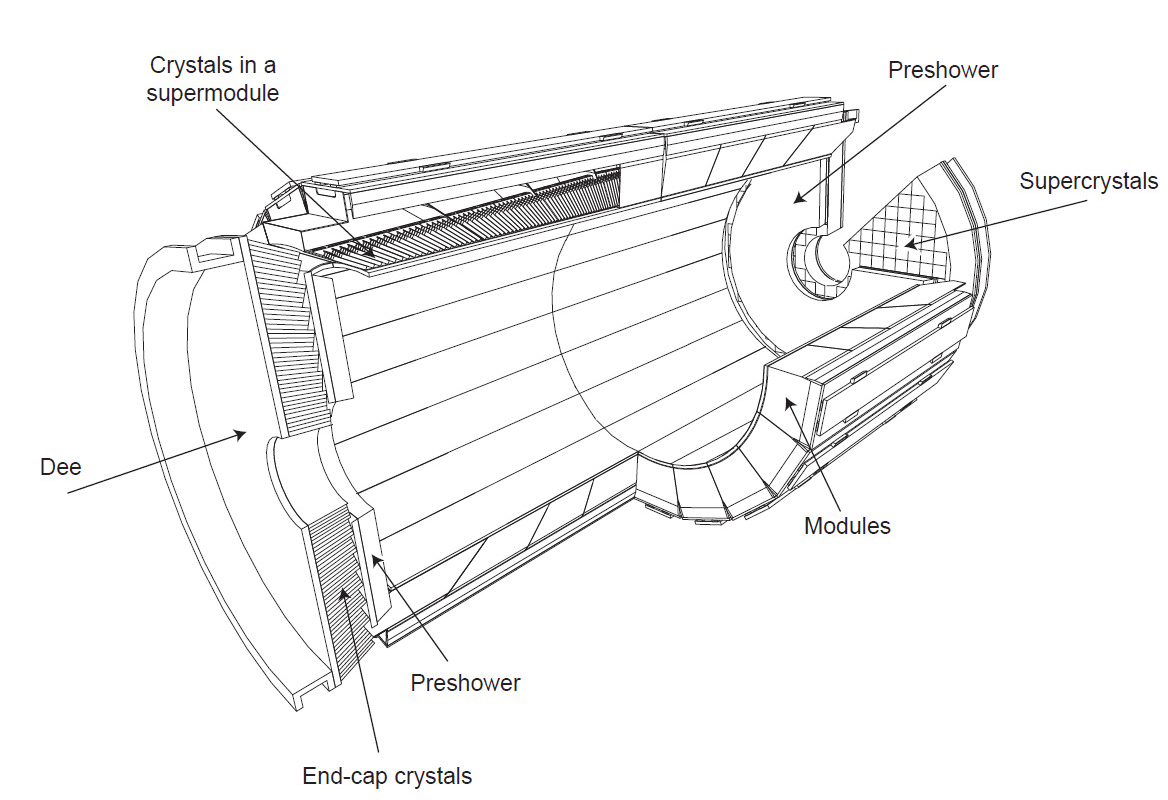
\includegraphics[width=\textwidth]{Figures/ECAL.png}
\caption{Geometric view of one quarter of the ECAL (top). Layout of the CMS electromagnetic calorimeter presenting the arrangement of crystal modules, supermodules, endcaps and the preshower in front (bottom) \cite{CMSexperiment}.}
\end{figure}

\begin{figure}\label{fig-ECALRapidity}
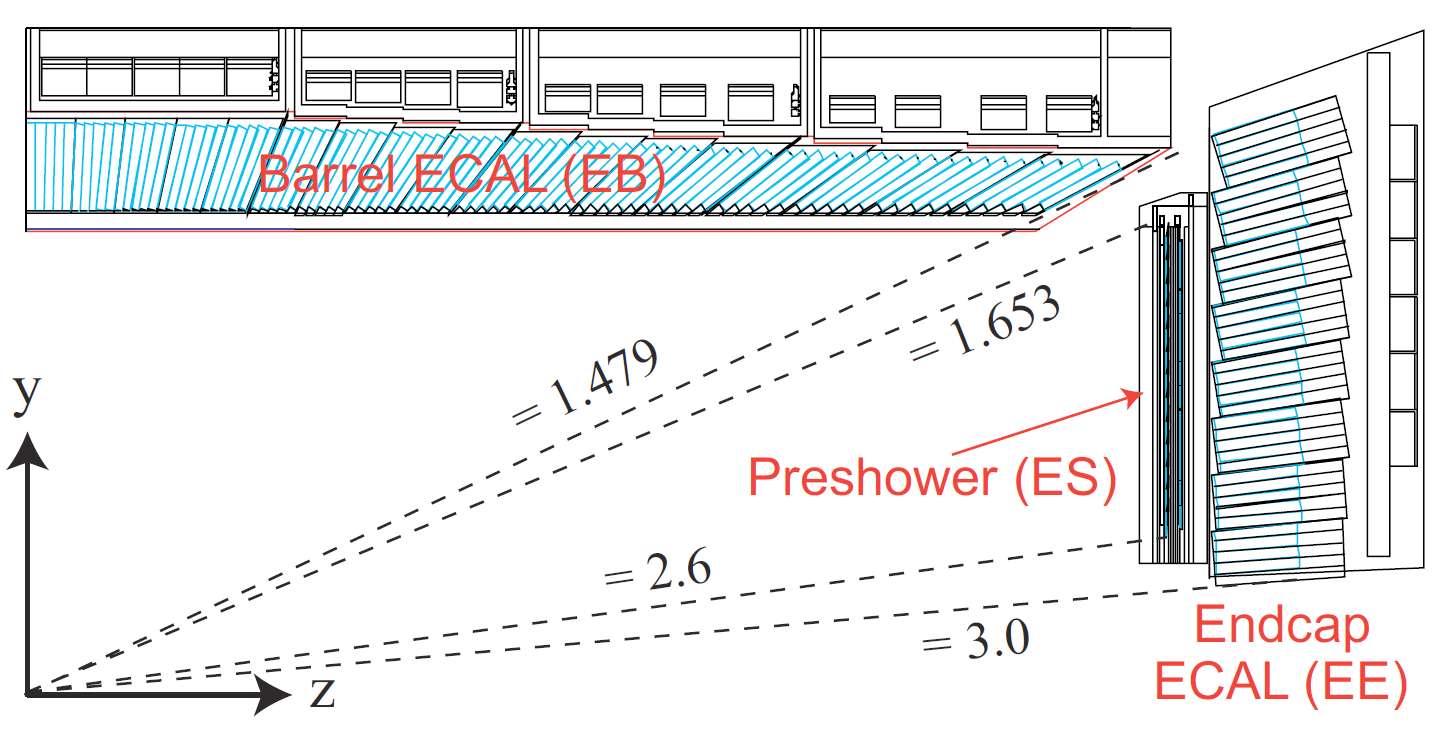
\includegraphics[width=\textwidth]{Figures/ECALRapidity.png}
\caption{Geometric view of one quarter of the ECAL (top). Layout of the CMS electromagnetic calorimeter presenting the arrangement of crystal modules, supermodules, endcaps and the preshower in front (bottom) \cite{CMSexperiment}.}
\end{figure}

\subsection{Hadron calorimeter} \label{subsec-HadronCalorimeter}

\subsection{Superconducting solenoid} \label{subsec-SuperconductingSolenoid}

\subsection{Muon system} \label{subsec-MuonSystem}

\begin{figure}\label{fig-CMSLongitudinalView}
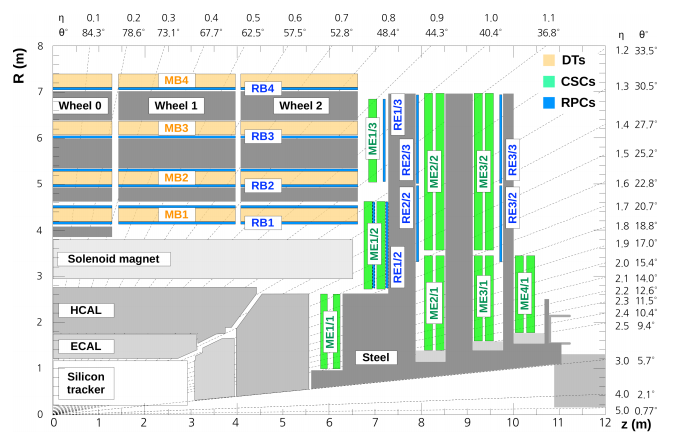
\includegraphics[width=\textwidth]{Figures/CMSLongitudinalView.png}
\caption{Layout of one quadrant of CMS. The figure shows the four DT stations in the barrel (MB1-MB4, yellow), the four CSC stations in the endcap (ME1-ME4, green), and the RPC stations (RB1-RB4 and RE1-RE3) \cite{CMSexperiment}.}
\end{figure}

\subsection{Trigger} \label{subsec-Trigger}

\subsection{Particle reconstruction} \label{subsec-ParticleReconstruction}
